\chapter{Robust Android Malware Familial Classification}
\thispagestyle{chapterfancy}


Our first objective for this thesis is to test the results obtained by Wu \textit{et al.} in their paper "Contrastive Learning for Robust Malware Familial Classification" \cite{wu2022contrastive}. \\
Once thoroughly explained how the system works, we'll show how we were able to replicate it by presenting the codes written and some intermediate  results to better explain the process. Once this is done, in the next chapter the focus will shift on applying the ideas presented in the paper on a different environment: Linux IoT.

\section{Motivation}

Being the most widely used mobile operating system and due to its open-source nature and market openness, Android has been the main target of malware attacks for years \cite{kivva2023itthreat}. \\
To be able to hide their malicious tasks, different code obfuscation techniques have been applied by attackers \cite{dong2018understanding}. After obfuscation, malware samples become more difficult to analyze and even samples from the same family may appear different from each other if different obfuscation techniques have been applied. \\
Most traditional Android malware analysis methods cannot resist code obfuscation. Android malware familial classifiers can be mainly divided in two categories: string-based and graph-based. The first methods usually focus on permission requested by apps and search for the presence of strings (\textit{e.g.}, API calls) inside the disassembled code to build models to analyze Android malware, but can be usually easily evaded by obfuscation due to their lack of structural and contextual information of the program behaviour. On the other hand, graph-based methods distill the program semantics of apps into graph representations and apply graph matching to analyze the malware families. However, as shown by Dong \textit{et al.} \cite{dong2018understanding}, more often than not malware creators perform complex obfuscations (\textit{e.g.}, control-flow obfuscation) to hide their malicious objectives, hindering the results of the models by rendering useless many of the features extracted with these methods. \\
To address this issue, Wu \textit{et al.} \cite{wu2022contrastive} propose the use of contrastive learning, due to its powerful high level feature extraction and its many successful applications in other fields (\textit{e.g.}, text representation learning and language understanding). 

\section{System Architecture}

In this section we'll show how \textit{IFDroid}, the contrastive learning-based robust and interpretable Android malware classification system proposed by Wu \textit{et al.} \cite{wu2022contrastive}, works. \\

\begin{figure}[H]
    \centering
    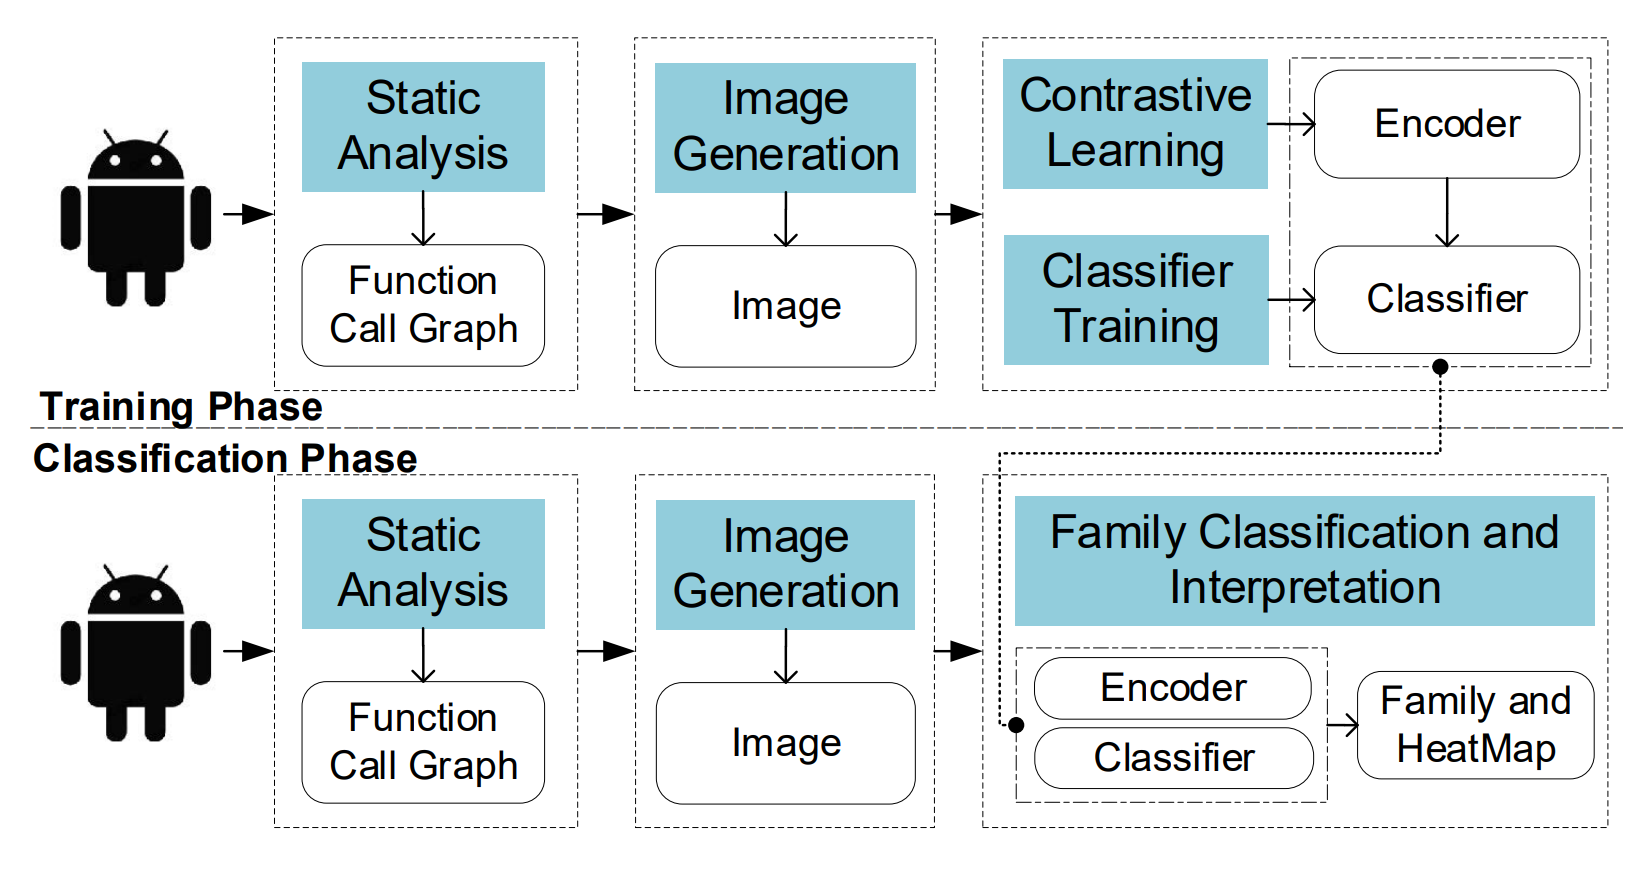
\includegraphics[width=0.75\linewidth]{Images/SOIFDroid.png}
    \caption{System Overview of \textit{IFDroid}.}
    \label{fig:SOIFDroid}
\end{figure}

\noindent As shown in Figure \ref{fig:SOIFDroid}, \textit{IFDroid} consists of two main phases: the Training Phase and the Classification Phase. \\
During the Training Phase we aim to train a robust encoder (via Contrastive Learning) and a classifier. To do so we follow four steps:

\begin{enumerate}
    \item \textbf{Static Analysis}: the Function Call Graph (FCG) is extracted from the malware using a software called Androguard \cite{desnos2011androguard} where every node is either an API call or a user-defined function (UDF).
    \item \textbf{Image Generation}: the FCG is transformed into an image using centrality measures as pixels.
    \item \textbf{Contrastive Learning}: an encoder based on a ResNet18 Neural Network with a SupConLoss is trained using the generated images as input.
    \item \textbf{Classifier Training}: a classifier is trained using the encoded images as input.
\end{enumerate}

\noindent During the Classification Phase we use the trained model to classify unlabeled malware into their corresponding families.

\subsection{Static Analysis}
It has been empirically demonstrated that graph representation is more robust than string-based features \cite{fan2018android}, therefore \textit{IFDroid} performs low-cost program analysis (\textit{e.g.}, context- and flow-insensitive analysis) to distill the program semantics of a malware sample into a function call graph. To do so, a widely used reverse engineering tool named Androguard \cite{desnos2011androguard} is used to perform the Static Analysis.

\begin{figure}[H]
    \centering
    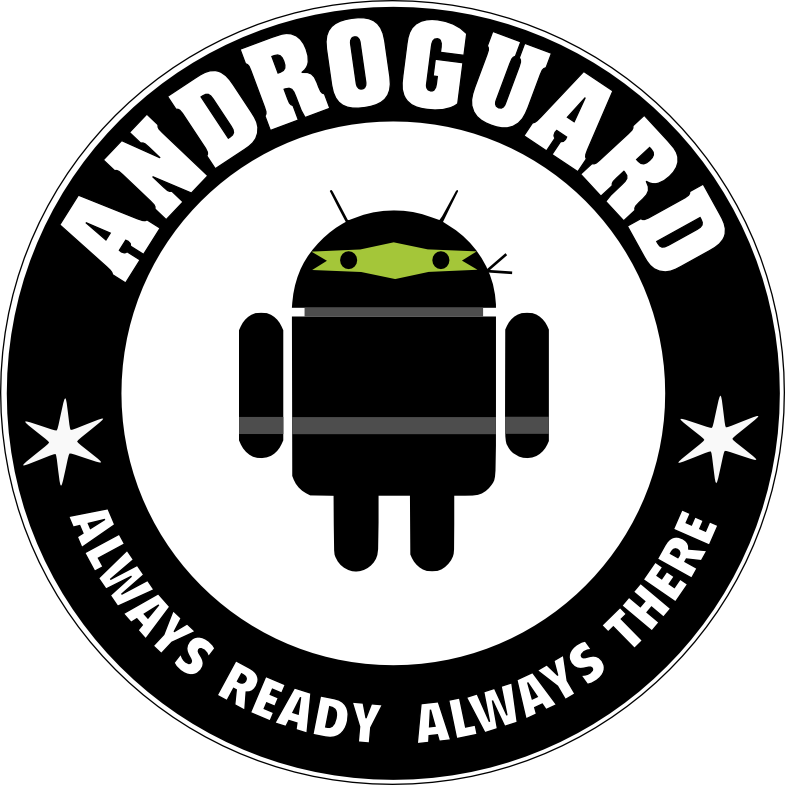
\includegraphics[width=0.4\linewidth]{Images/AndroguardLogo.png}
    \caption{Androguard Logo.}
    \label{fig:AndroLogo}
\end{figure}

\subsection{Image Generation}

Deep-learning based image classification has been object of research for several decades and can now process millions of images while maintaining high accuracy. Furthermore, its output can be visualized to give a better intuition to users. Because of these advantages, image-based methods have been widely employed in malware analysis. However, most of these approaches \cite{nataraj2011malware} use semantic-insensitive mapping algorithms (\textit{e.g.}, reshaping the binary as a 0-1 Matrix), reducing the accuracy of the model. \\
To achieve efficient and semantic-sensitive malware analysis, Wu \textit{et al.} propose the use of centrality analysis: a technique that checks the importance of a node in the graph by analyzing its centrality measures. For this model, four widely used centrality measures are selected:

\begin{enumerate}
    \item \textbf{Degree Centrality} \cite{freeman2002centrality} : assigns an importance score solely based on the number of edges of a node. The value is then normalized by the maximum possible degree in a graph $N-1$.  \\
    \begin{equation}
        C_{d}(i)=\frac{\operatorname{deg}(i)}{N-1}
    \end{equation}
    \item \textbf{Katz Centrality} \cite{katz1953new} : assigns an importance score based on the sum of the neighbours scaled by a constant that decreases based the further the neighbour is. $A^{k}$ is the adjacency matrix at distance $k$, while $\alpha$ is a constant between 0 and 1. The vector containing all the nodes' centralities is then normalized.  \\
    \begin{equation}
        C_{k}(i)=\sum_{k=1}^{\infty} \sum_{j=1}^{+\infty} \alpha^{k}\left(A^{k}\right)_{j i}
    \end{equation}
    \item \textbf{Closeness Centrality} \cite{freeman2002centrality} : assigns an importance score negatively correlated to the average of the shortest path length from the node to every other node in the graph normalized by the maximum possible path length in a graph $N-1$.  \\
    \begin{equation}
        C_{c}(i)=\frac{N-1}{\sum_{i \neq j} d(i, j)}
    \end{equation}
    \item \textbf{Harmonic Centrality} \cite{marchiori2000harmony} : assigns an importance score based on the reciprocal of the harmonic mean of the distances from a node to all other nodes in the graph.  \\
    \begin{equation}
        C_{h}(i)=\frac{\sum_{i \neq j} \frac{1}{d(i, j)}}{N-1}
    \end{equation}
\end{enumerate}

\noindent To generate the image, for every node taken into consideration all four centrality measures are calculated and then written into a vector. That vector is then reshaped into a square grayscale image by padding the extra pixels with zeros (\textit{i.e.}, black pixels). \\
The main objective now is how to select which nodes to take into consideration.

\subsubsection{Sensitive APIs Selection} 
Android apps use API calls to access operating system functionality and system resources. On the other hand, malware samples tend to invoke sensitive APIs to perform malicious tasks. For example, \textit{getDeviceID} can get your phone’s IMEI and \textit{getLine1Number} can obtain your phone number. \\
Gong \textit{et al.} \cite{gong2020experiences} showed that, out of the >50k API calls provided by the current Android SDK (Software Developer Kit), there are 426 that have a high correlation to malicious behaviour. To find this subset, they used \textit{Spearman’s rank correlation coefficient} (SRC \cite{spearman1904proof}) to evaluate the statistical correlation between an API call and the malice of apps. Their API selection approach consists of four steps:

\begin{itemize}
    \item \textbf{Step 1. Selecting APIs with the highest correlation with malware}: using SRC, it tracks the APIs with $|SRC|\geq0.2$. Out of all of these, many of them are seldom invoked by the apps in our dataset (invoked by fewer than 0.1\% apps). Using these infrequently invoked APIs as features may bring over-fitting problems to machine learning, and thus the API selector has to neglect these. After Step 1, we have a total of 260 APIs that satisfy the requirements.
    \item \textbf{Step 2. Selecting APIs that relate to restrictive permissions}: to protect the privacy/security of user information, an app needs to request permissions before obtaining certain information or fulfilling certain functions. Android permissions are classified into three protection levels: normal, signature, and dangerous. The APIs protected by dangerous-level permissions and those by signature level permissions are oftentimes relevant to sensitive user data (such as camera, SMS, and location data), which are thus crucial for malware detection. The API selector takes advantage of the Axplorer \cite{backes2016demystifying} and PScout \cite{au2012pscout} tools to select the APIs related to restrictive permissions. After Step 2, we have a total of 112 APIs that satisfy the requirements.
    \item \textbf{Step 3. Selecting APIs that perform sensitive operations}: the third strategy selects APIs that perform sensitive operations. there are five categories of sensitive operations commonly exploited for conducting attacks: (1) APIs that can lead to privilege escalation, (\textit{e.g.}, shell command execution) APIs, (2) APIs for database operations and file read/write, which are commonly used in privacy leakage attacks, (3) APIs operating on key Android components, (\textit{e.g.}, those for creating an Android window or overlay), which are used in attacks such as Activity hijacking, (4) cryptographic operation APIs, which are commonly used in ransomware attacks, and (5) APIs for dynamic code loading, which can load malicious payloads at runtime and perform attacks such as update attack. After Step 3, we have a total of 70 APIs that satisfy the requirements.
    \item \textbf{Step 4. Combining the above}: The last step is combining the above strategies, leading to a total of 426 key APIs (after removing duplicates).
\end{itemize}

\subsection{Contrastive Learning}
The goal of contrastive learning is to maximize the agreement between original data and its positive data while minimize the agreement between original data and its negative data by using a contrastive loss in the vector space.

\begin{figure}[H]
    \centering
    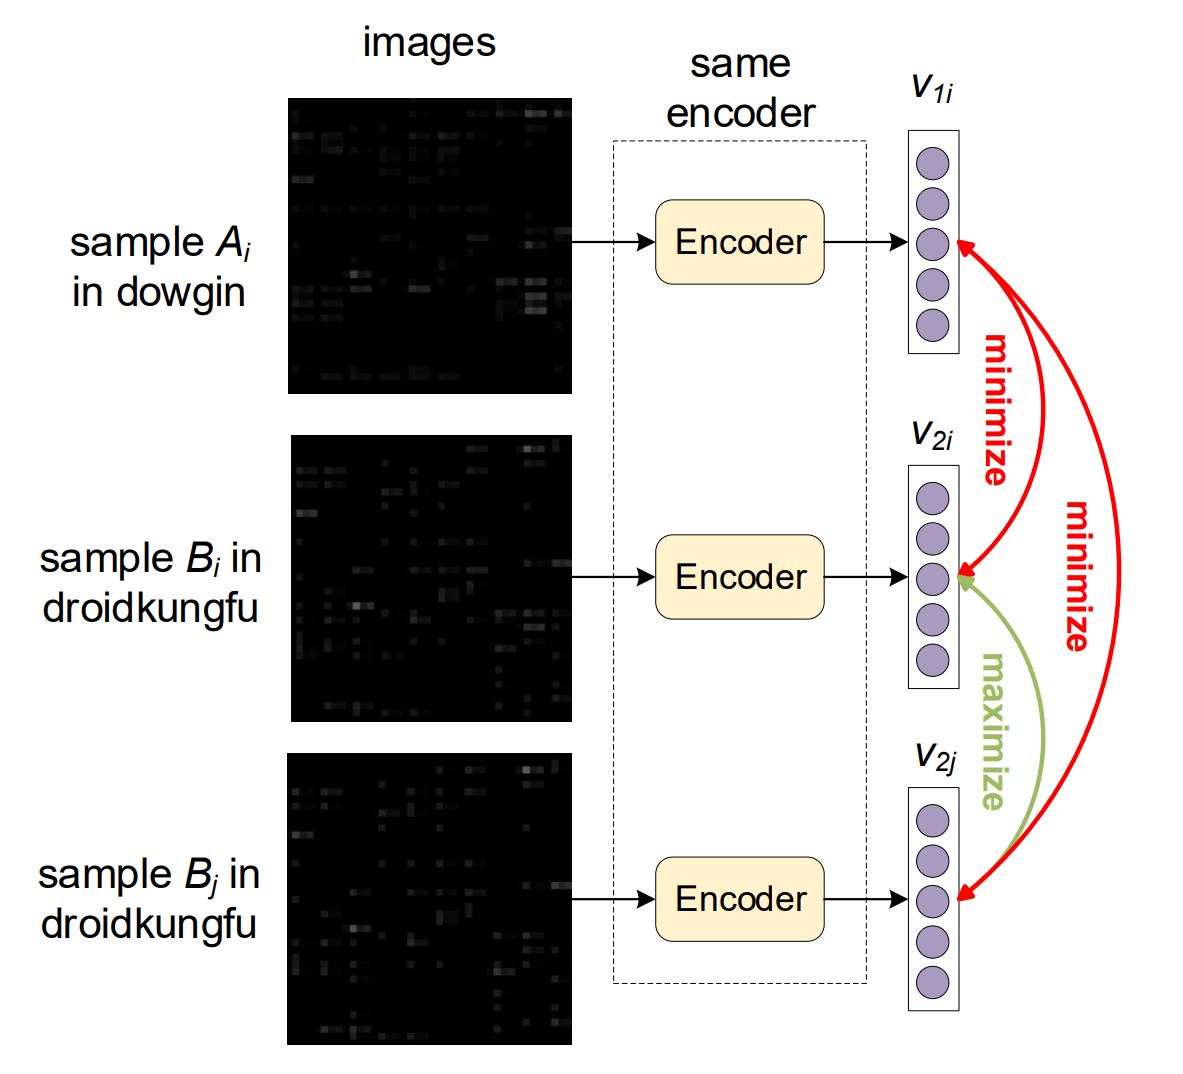
\includegraphics[width=0.6\linewidth]{Images/Encoder.png}
    \caption{Supervised contrastive learning in \textit{IFDroid}.}
    \label{fig:Encoder}
\end{figure}

\noindent It was found by Khosla \textit{et al.} \cite{khosla2020supervised} that the label information of samples can be used to improve the accuracy of contrastive learning, therefore supervised contrastive learning is selected to train \textit{IFDroid}'s encoder. \\
The loss used to train the encoder (SupConLoss) calculates the contrastive loss in batches. Given an input batch of data, SupConLoss works as the following: 

\begin{equation}
    \mathcal{L}_{\text {out }}^{\text {sup }}=\sum_{i \in I} \frac{-1}{|P(i)|} \sum_{p\in P(i)} \log \frac{\exp \left(v_{i} \cdot v_{p} / \tau\right)}{\sum_{a\in A(i)} \exp \left(v_{i} \cdot v_{a} / \tau\right)}
    \label{eq:SupConLoss}
\end{equation}

\vspace{1.5pt}
\noindent where $I$ is the set of indices of the inputs, $v_{i}$ represents the embedding of the input $x_{i}$, $\tau\in\mathbb{R}^{+}$ is a scalar temperature parameter, $A(i)\equiv I\backslash\{i\}$, $P(i)\equiv \{p\in A(i) : l_{p} = l_{i}\}$ is the set of indices of all positives in the batch apart from $i$ ($l_{i}$ is the label of $x_{i}$) and $|P(i)|$ is its cardinality. It uses the positive normalization factor (\textit{i.e.}, $\frac{1}{|P(i)|}$)
to remove bias present in multiple positives samples and preserve the summation over negatives in the denominator to increase performance.

\begin{table}[H]
    \centering
    \begin{tabular}{|c|c|}
        \hline
        Parameters & Settings \\
        \hline
        loss function & SupConLoss in \cite{khosla2020supervised} \\
        temperature & 0.07 \\
        optimizer & SGD \\
        momentum & 0.9 \\
        weight decay & 0.0001 \\
        learning rate & 0.05 \\
        batch size & 64 \\
        epoch & 100 \\
        \hline
    \end{tabular}
    \caption{Paramaters used in \textit{IFDroid} contrastive learning}
    \label{tab:IFDroidParam}
\end{table}

\noindent The authors chose ResNet18 \cite{he2016deep} as the image encoder after experimenting with many widely-used neural networks, since it can achieve a balance between accuracy and efficiency. \\
By applying centrality analysis on the 426 sensitive APIs discussed in the previous section, the input of \textit{IFDroid} becomes a 42*42 pixel grayscale image (with the last 60 pixels black, since $42*42-426*4=60$). Since the inputs in most computer vision datasets are 224*224 pixels RGB images, to make ResNet18 suitable for the inputs generated by this model it needs to be modifies so that the dimension of the input is the same
as the size of its image. \\
Table \ref{tab:IFDroidParam} shows the details of parameters used in \textit{IFDroid} contrastive learning. The loss function is the
same as in \cite{khosla2020supervised}, namely Supervised Contrastive Loss. The whole procedure is trained using Stochastic Gradient Descent (SGD) with 0.9 momentum and 0.0001 weight decay. The output in this step is a learned encoder that can convert an image into a vector whose dimension is 512.

\subsection{Classifier Training}

In this step, the trained encoder is used to obtain the inputs for the classifier, a one-layer fully connected neural network that uses Cross Entropy Loss to correctly sort the input malware sample into their label. The output of the classifier is a n-tuple where n is the number of different labels possible. The Cross Entropy Loss works as the following:

\begin{equation}
    \mathcal{L}_{c e}=-\sum_{i \in I} \log \frac{\exp \left(x_{i,l_{i}}\right)}{\sum_{c\in C} \exp \left(x_{i,c}\right)}
    \label{eq:CrossEntropy}
\end{equation}

\vspace{1.5pt}
\noindent where $I$ is the set of indices of the inputs, $C$ is the set of possible labels, $x_{i,c}$ is the value of the output for the label $c$ and $l_{i}$ is the correct label of the input $x_{i}$.

\begin{figure}[H]
    \centering
    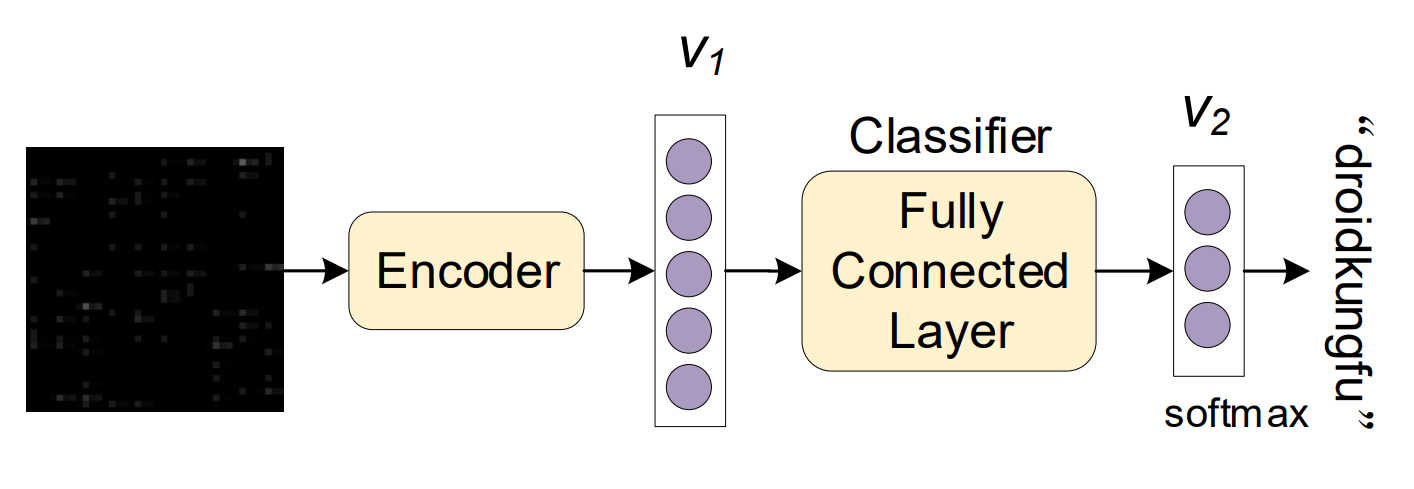
\includegraphics[width=0.7\linewidth]{Images/Classifier.png}
    \caption{Familial classification of \textit{IFDroid}.}
    \label{fig:Classifier}
\end{figure}

\section{Our Experiment}
Before applying the ideas behind \textit{IFDroid} to Linux IoT malware classification, we want to re-create the experiments performed by Wu \textit{et al.} \cite{wu2022contrastive}, as to check the replicability of their results.

\subsection{Obtaining the Malware Samples}
To be able to train our neural network, we first need a Dataset to work on. Following the original paper, we land on AndroZoo \cite{allix2016androzoo}, a growing collection of Android Applications collected from several sources, including the official Google Play app market. It currently contains 24,264,358 different APKs\footnote{as of 2024-02-07.}, each of which has been (or will soon be) analysed by tens of different AntiVirus products to know which applications are detected as Malware \cite{allix2024androzooweb}.

\subsubsection{AndroZoo}
This dataset presents a huge collection of APKs collected from different sources such as Google Play, Anzhi, AppChina and many others. It was created by using a dedicated web crawler using the scrapy framework, a fast high-level web crawling and scraping framework for Python. Every candidate app which was available for free run through a processing pipeline that:

\begin{enumerate}
    \item Ensured that app had not already been downloaded;
    \item Downloads the file;
    \item Computes its SHA256 checksum;
    \item Archives the file.
\end{enumerate}

\noindent The obtained APKs are then classified using Euphony \cite{hurier2017euphony}, a tool to infer a single label of a malicious application from a list of VirusTotal reports. \\ 
After being granted access to the dataset, we obtained an API key. With this API key we were able to download any APK inside of the dataset simply providing its SHA256, which represents the hash value of a malware sample and is used to uniquely identify files, in the following way:

\begin{center}
    \fbox{https://androzoo.uni.lu/api/download?apikey=\$\{APIKEY\}\&sha256=\$\{SHA256\}}
\end{center}

\vspace{1.5pt}
\noindent Using a simple Python script, iterating over the list of SHA256s provided by the AndroZoo team, we were able to download the needed samples. \\
Due to storage and time deficiency, we reduced our dataset to 5000 samples, equally divided between 5 malware families: \textsc{Airpush}, \textsc{Droidkungfu}, \textsc{Feiwo}, \textsc{Utchi} e \textsc{Wooboo}. \\
These malware families are all Adware, \textit{i.e.} a type of malware that displays or downloads advertising material on the system, except for \textsc{Droidkungfu}, which is a Trojan malware that forwards confidential details to a remote server.

\subsection{Extracting the Function Call Graph}
After obtaining the samples, it's time to extract the Function Call Graph (FCG) from the APKs. To reach this objective, we'll use the same tool used for \textit{IFDroid}, \textit{i.e.} Androguard \cite{desnos2011androguard}.

\subsubsection{Androguard}
Androguard is an open-source, Python-based security tool designed for analyzing and reverse engineering Android applications. The specific command we are going to use is "androguard cg", which creates a Call Graph from APK and exports it in .gml format, a simple text-based file format used to represent graph structures. The command works as the following: 

\begin{center}
\begin{lstlisting}[style=androguard]
Usage: androguard cg [OPTIONS] APK

  Create a call graph and export it into a graph format.

  The default is to create a file called callgraph.gml in the current directory!

  classnames are found in the type "Lfoo/bar/bla;".

  Example:

      $ androguard cg examples/tests/hello-world.apk

Options:
  -o, --output TEXT           Filename of the output file,
                              the extension is used to 
                              decide which format to use  
                              [default: callgraph.gml]
  -s, --show                  instead of saving the graph, 
                              print it with mathplotlib 
                              (you might not see anything!)
  -v, --verbose               Print more output
  --classname TEXT            Regex to filter by classname  
                              [default: .*]
  --methodname TEXT           Regex to filter by methodname  
                              [default: .*]
  --descriptor TEXT           Regex to filter by descriptor  
                              [default: .*]
  --accessflag TEXT           Regex to filter by accessflags  
                              [default: .*]
  --no-isolated / --isolated  Do not store methods which has 
                              no xrefs
  --help                      Show this message and exit.
\end{lstlisting}
\end{center}

\noindent We use this tool on our 5000 samples to obtain their FCGs in .graphml format, which is more suitable than .gml for complex graphs like the ones we are creating. To better show the complexity of the graphs generated in this way, in Figure \ref{fig:WoobooGraph} is presented the FCG of the smallest \textsc{Wooboo} sample out of the 1000 we used, rendered using Gephi \cite{bastian2009gephi}, a open-source software for the visualization and exploration of all kinds of graphs and networks, using the Fruchterman Reingold layout \cite{fruchterman1991graph}.

\begin{figure}[H]
    \centering
    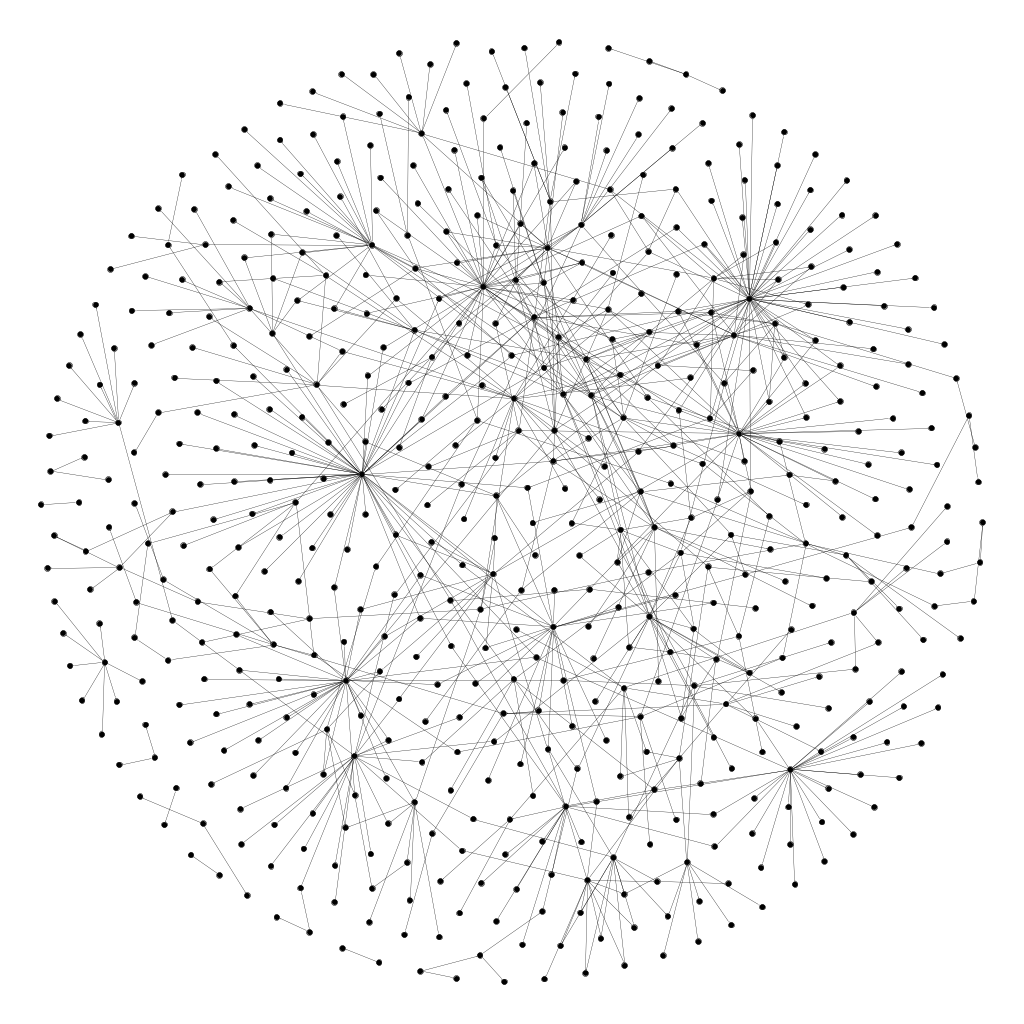
\includegraphics[width=0.8\linewidth]{Images/WoobooGraph.png}
    \caption{Function Call Graph of a \textsc{Wooboo} malware sample, rendered using Gephi with the Fruchterman Reingold layout.}
    \label{fig:WoobooGraph}
\end{figure}

\subsection{Centrality Analysis}
Now it's time to perform Centrality Analysis on the sensitive APIs present inside the extracted graphs. To do so, we use NetworkX \cite{hagberg2008exploring}, a Python package for the creation, manipulation, and study of the structure, dynamics, and functions of complex networks.

\subsubsection{NetworkX}
This Python package has built-in functions to compute the four centrality measures we are after:

\begin{itemize}
    \item\fbox{degree\_centrality($G$)} \\
    \item\fbox{\parbox{0.83\textwidth}{katz\_centrality($G,\, alpha=0.1,\, beta=1.0,\, max\_iter=1000,\, tol=1e-06,\\ nstart=None,\, normalized=True,\, weight=None$)}} \\
    \item\fbox{closeness\_centrality($G,\, u=None,\, distance=None,\, wf\_improved=True$)} \\
    \item\fbox{harmonic\_centrality($G,\, nbunch=None,\, distance=None,\, sources=None$)}
\end{itemize}

\vspace{1.5pt}
\noindent where $G$ represents the input graph, $alpha$ is an attenuation factor, $beta$ is a weight attributed to the immediate neighborhood, $max\_iter$ is the maximum number of iterations, $tol$is the error tolerance used to check convergence, $wf\_improved$ makes the algorithm use the Wassermann and Faust improved formula \cite{wasserman1994social}. \\
Since Wu \textit{et al.} haven't specified any parameters for the  measures, we'll use the default settings for our tests. For the harmonic centrality normalization is also needed, since the NetworkX package doesn't perform it automatically. \\
By writing a simple Python script we computed the centrality measures of the sensitive APIs in our input graphs and generated and exported 5000 matrix (our images) using the Numpy package \cite{harris2020array}.

\subsection{Contrastive Learning}
To be able to replicate \textit{IFDroid}, we first need to create the custom ResNet18 that supports grayscale 42*42 pixels images, and then we need to write the Supervised Contrastive Loss \cite{khosla2020supervised} function. \\
To achieve this we used the PyTorch Python package \cite{paszke2019pytorch}, an open-source deep learning framework that is widely used for developing and training artificial neural networks.

\subsubsection{ResNet18}
The first difference between a standard ResNet18 and our embedder is the number of channels of the image. To solve this, we pass $image\_channels$ as a variable, so that the first Convolutional Layer has the correct number of $in\_channels$. \\
The second difference is in the last layer: normally a ResNet18 ends with a Linear Layer that transforms the high-level features extracted by the convolutional layers into class scores. But since we are training an embedder, we don't need this final step and instead we normalize the 512 tensor generated by layer4. \\
The difference in size is already taken into account in the original code, thanks to the $AdaptiveAvgPool2d$ at the end of the model. \\

\pagebreak 

\begin{lstlisting}[style=mypython, xleftmargin=.03\textwidth, xrightmargin=.03\textwidth]
class ResNet_18(nn.Module):
    
    def __init__(self, image_channels):
        
        super(ResNet_18, self).__init__()
        self.in_channels = 64
        self.conv1 = nn.Conv2d(image_channels, 64, kernel_size=7, 
                               stride=2, padding=3, device=device)
        self.bn1 = nn.BatchNorm2d(64, device=device)
        self.relu = nn.ReLU()
        self.maxpool = nn.MaxPool2d(kernel_size=3, stride=2, 
                                    padding=1)
        
        self.layer1 = self.__make_layer(64, 64, stride=1)
        self.layer2 = self.__make_layer(64, 128, stride=2)
        self.layer3 = self.__make_layer(128, 256, stride=2)
        self.layer4 = self.__make_layer(256, 512, stride=2)
        
        self.avgpool = nn.AdaptiveAvgPool2d((1, 1))
        
    def __make_layer(self, in_channels, out_channels, stride):
        
        identity_downsample = None
        if stride != 1:
            identity_downsample = self.identity_downsample(in_channels, 
                                                           out_channels)
            
        return nn.Sequential(
            Block(in_channels, out_channels, 
                  identity_downsample=identity_downsample, 
                  stride=stride), 
            Block(out_channels, out_channels)
        )
        
    def forward(self, x):
        
        x = self.conv1(x)
        x = self.bn1(x)
        x = self.relu(x)
        x = self.maxpool(x)
        
        x = self.layer1(x)
        x = self.layer2(x)
        x = self.layer3(x)
        x = self.layer4(x)
        
        x = self.avgpool(x)
        x = x.view(x.shape[0], -1)
        return nn.functional.normalize(x.squeeze(0), dim=0)
    
    def identity_downsample(self, in_channels, out_channels):
        
        return nn.Sequential(
            nn.Conv2d(in_channels, out_channels, kernel_size=1, stride=2, 
                      padding=0, device=device), 
            nn.BatchNorm2d(out_channels, device=device)
        )
\end{lstlisting}

\begin{lstlisting}[style=mypython, xleftmargin=.03\textwidth, xrightmargin=.03\textwidth]
class Block(nn.Module):
    
    def __init__(self, in_channels, out_channels, 
                 identity_downsample=None, stride=1):
        super(Block, self).__init__()
        self.block = nn.Sequential(nn.Conv2d(in_channels, out_channels, 
                                   kernel_size=3, stride=stride, 
                                   padding=1, device=device),
                                   nn.BatchNorm2d(out_channels, 
                                   device=device),
                                   nn.Conv2d(out_channels, out_channels, 
                                   kernel_size=3, stride=1, padding=1, 
                                   device=device),
                                   nn.BatchNorm2d(out_channels, 
                                   device=device)
                                  )
        self.relu = nn.ReLU()
        self.identity_downsample = identity_downsample
        
    def forward(self, x):
        identity = x
        x = self.block(x)
        if self.identity_downsample is not None:
            identity = self.identity_downsample(identity)
        x += identity
        x = self.relu(x)
        return x
\end{lstlisting}

\subsubsection{Supervised Contrastive Loss}
Now that we've written the code for the embedder, the next stop is to define the loss function. As previously stated, we are gonna employ the Supervised Contrastive Loss defined by Khosla \textit{et al.} \cite{khosla2020supervised}. \\

\begin{lstlisting}[style=mypython, xleftmargin=.03\textwidth, xrightmargin=.03\textwidth]
class SupConLoss(nn.Module):
    def __init__(self, temperature=0.07):
        super(SupConLoss, self).__init__()
        self.temp = temperature

    def forward(self, features, labels):
        loss = 0
        for i in range(0, len(labels)):
            denom_sum = 0
            for j in range(0, len(labels)):
                if i != j:
                    denom_sum += torch.exp(torch.dot(features[i],
                                                     features[j])/
                                                     self.temp)
            mid_sum = 0
            positives = 0
            for j in range(0, len(labels)):
                if i != j and labels[i] == labels[j]:
                    mid_sum += torch.log(torch.exp(torch.dot(features[i],
                                                             features[j])
                                                             /self.temp)
                                                             /denom_sum)
                    positives += 1
            if positives>0:
                loss += mid_sum*(-1)/positives
        
        return loss/len(labels)
\end{lstlisting}

\noindent This is a simple PyTorch implementation of the Equation \ref{eq:SupConLoss}. The only difference being the normalization performed on the return line, so that the loss value doesn't depend on the batch size.

\subsection{Results}
It's now time to train our model. We used both a NVIDIA Tesla T4 (provided by Leonardo S.p.A.) and a NVIDIA GeForce RTX 3050 interchangeably for this experiment. \\
As indicated by Wu \textit{et al.} \cite{wu2022contrastive}, we train both our encoder and classifier for 100 epochs. At epoch 0, the encoder has a train loss of 4.09590 and a validation loss of 4.09241, while at epoch 99 it has a train loss of 2.69575 and a validation loss of 3.06028. Our classifier, on the other hand, at epoch 0 has a train loss of 1.61223 and a validation loss of 1.61022, while at epoch 99 it has a train loss of 0.78163 and a validation loss of 0.71369. \\

\begin{figure}[H]
    \centering
    \begin{subfigure}{0.45\textwidth}
        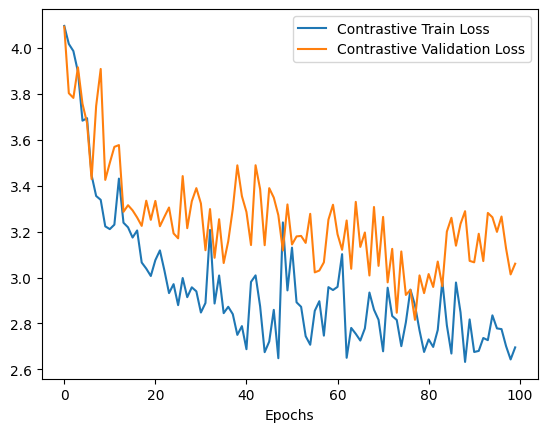
\includegraphics[width=\linewidth]{Images/ConLoss_5.png}
        \caption{Encoder Loss}
        \label{fig:ConLoss}
    \end{subfigure}
    \hfill
    \begin{subfigure}{0.45\textwidth}
        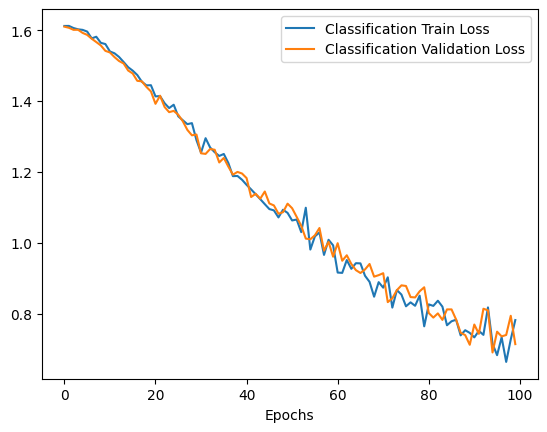
\includegraphics[width=\linewidth]{Images/ClassLoss_5.png}
        \caption{Classifier Loss}
        \label{fig:ClassLoss}
    \end{subfigure}
    \caption{Variation of the Loss over the epochs for the Android encoder and classifier.}
    \label{fig:Loss}
\end{figure}

\noindent To measure the effectiveness of our model, we leverage some widely used metrics (Table \ref{tab:Metrics}) to then compare them to \textit{IFDroid} results.

\begin{table}[H]
    \centering
    \resizebox{\linewidth}{!}{
    \begin{tabular}{|c|c|c|}
        \hline
        \textbf{Metrics} & \textbf{Abbr} & \textbf{Definition} \\
        \hline
        True Positive & \textbf{TP} & \#malware in family $f$ are correctly classified into family $f$ \\
        True Negative & \textbf{TN} & \#malware not in family $f$ are correctly not classified into family $f$ \\
        False Positive & \textbf{FP} & \#malware not in family $f$ are incorrectly classified into family $f$ \\
        False Negative & \textbf{FN} & \#malware in family $f$ are incorrectly not classified into family $f$ \\
        True Positive Rate & \textbf{TPR} & $TP/(TP+FN)$ \\
        False Negative Rate & \textbf{FNR} & $FN/(TP+FN)$ \\
        True Negative Rate & \textbf{TNR} & $TN/(TN+FP)$ \\
        False Positive Rate & \textbf{FPR} & $FP/(TN+FP)$ \\
        Precision & \textbf{P} & $TP/(TP+FP)$ \\
        Recall & \textbf{R} & $TP/(TP+FN)$ \\
        F-measure & \textbf{F1} & $2*P*R/(P+R)$ \\
        Classification Accuracy & \textbf{CA} & $(TP+TN)/(TP+TN+FP+FN)$ \\
        \hline
    \end{tabular}
    }
    \caption{List of the various metrics used in this experiment.}
    \label{tab:Metrics}
\end{table}

\noindent Wu \textit{et al.} only provided the F-measure of \textit{IFDroid} in their paper \cite{wu2022contrastive}. We were able to find, in an older version of the same paper \cite{wu2021obfuscation}, the True Positive Rate and False Positive Rate of the malware classification, but it must be kept in mind that represents an older build of \textit{IFDroid}, and it doesn't accurately represent its full capabilities. In Table \ref{tab:IFDroidVS} the F1Scores are from the newer version, while the TPR and FPR are from the older one. \\

\begin{table}[H]
    \centering
    %\resizebox{\linewidth}{!}{
    \begin{tabular}{|c|cc|cc|cc|}
        \hline
        \multirow{2}{3.5em}{\textbf{Family}} & \multicolumn{2}{c|}{\textbf{TPR(\%)}} & \multicolumn{2}{c|}{\textbf{FPR(\%)}} & \multicolumn{2}{c|}{\textbf{F1}} \\
        & \textit{IFDroid} & \textit{ours} & \textit{IFDroid} & \textit{ours} & \textit{IFDroid} & \textit{ours} \\
        \hline
        airpush & 85.5 & 100 & 0.1 & 2.5 & 92.5 & 95.2 \\
        droidkungfu & 98 & 90.0 & 0 & 0.6 & 99.5 & 93.5 \\
        feiwo & ? & 92.5 & ? & 0.6 & 94.4 & 94.9 \\
        utchi & 100 & 100 & 0 & 0 & 100 & 100 \\
        wooboo & ? & 92.5 & ? & 2.5 & 98.2 & 91.4 \\
        \hline
    \end{tabular}
    %}
    \caption{Result metrics of both the original and our tests of \textit{IFDroid}.}
    \label{tab:IFDroidVS}
\end{table}

\noindent Last but not least, we show the other metrics improvements of our model over the epochs. \\

\begin{figure}[H]
    \centering
    \begin{subfigure}{0.3\textwidth}
        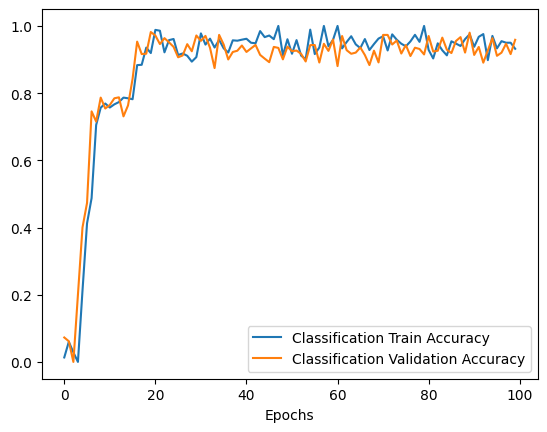
\includegraphics[width=\linewidth]{Images/Acc_5.png}
        \caption{Accuracy}
        \label{fig:Accuracy}
    \end{subfigure}
    \hfill
    \begin{subfigure}{0.3\textwidth}
        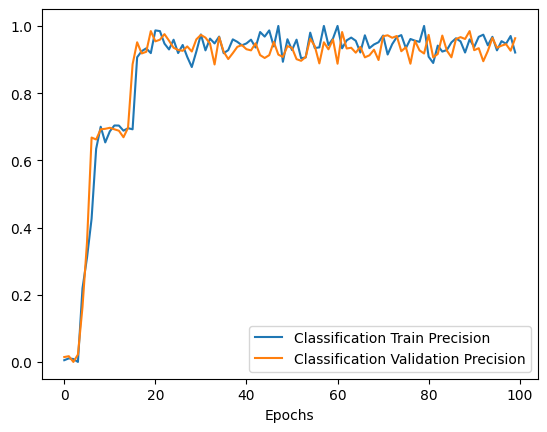
\includegraphics[width=\linewidth]{Images/Prec_5.png}
        \caption{Precision}
        \label{fig:Precision}
    \end{subfigure}
    \hfill
    \begin{subfigure}{0.3\textwidth}
        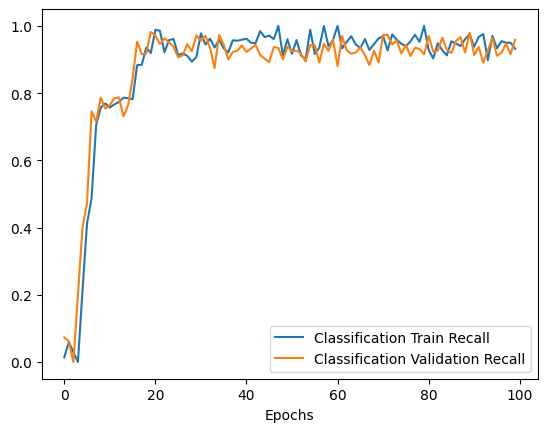
\includegraphics[width=\linewidth]{Images/Rec_5.png}
        \caption{Recall}
        \label{fig:Recall}
    \end{subfigure}
    \caption{Variation of different effectiveness metrics over the epochs for the Android classifier.}
    \label{fig:Metrics}
\end{figure}

\section{Conclusions}
Even with a smaller dataset, we were able to witness the capabilities of \textit{IFDroid}. It must be stated that the classifier was still trainable for many more epochs without risk of overfitting, but we decided to use the exact same variables as the original paper for the sake of this Thesis. \\
Regardless, the ideas shown in this Chapter are much more general than it could seem. Training an encoder using Supervised Contrastive Learning can be used with any kind of input, not only images. Many common classification methods may benefit from contrastive learning, such as:

\begin{itemize}
    \item \textbf{Binary-based methods}: Executable files, or binaries, are binary files containing machine code for the computer to execute. The binary carries all necessary information that enables the program’s execution in the target environment. Most of the works using this method take in byte sequences as input features for the learning models, resulting in very fast feature extraction but also making them susceptible to simple obfuscations techniques.
    \item \textbf{Opcode-based methods}: An opcode, abbreviated from operation code, is the portion of a machine language instruction specifying the operation to be performed. Opcode sequences, as the output of many reverse engineering tools, carry fine-grained information about the execution logic of the program. Due to the extremely fine granularity of opcode, a graph representation yielded by opcode may show a size rendering fast analysis impossible. Integrating opcode as function calls (blocks of opcodes that realize particular functionalities) can not only significantly reduce the size for graph representation but also result in improved modeling of the malware behavior at a higher level.
    \item \textbf{Graph-based methods}: The malicious behavior of malware can be characterized by certain components in some representative structures obtained from malware binaries that reflect the execution logic of the program. In the literature, Control Flow Graphs (CFGs) and Function Call Graphs (FCGs) are among the most widely adopted representative structures to serve this purpose. By extracting the vector representations of the semantics in the graph through graph embedding, we can capture essential discriminating information from malware samples.
    \item \textbf{API-based methods}: Application programming interface (API), a software interface that offers a service to other pieces of software, is used in high-level programming to invoke system calls at the low level. as far as dynamic analyses are concerned, API sequences captured during the program’s execution time are reported as the most significant data type that facilitates malware analysis.
\end{itemize}

\noindent Many other types of information can be obtained from static analysis and serve as behavioural indicators of malware.